\documentclass[10pt,aspectratio=169]{ntuabeamer}

\usepackage{booktabs}
\usepackage{tikz}
\usetikzlibrary{arrows.meta,positioning,fit}

\graphicspath{{assets/}{assets/generated/}}

\definecolor{softblue}{HTML}{5B8DB8}
\definecolor{softteal}{HTML}{63A6A0}
\definecolor{softgold}{HTML}{D7A85E}
\definecolor{softcoral}{HTML}{C77C6B}
\definecolor{softpurple}{HTML}{8B82A8}
\definecolor{softink}{HTML}{263746}

\framesource{lecun1998}{LeCun et al. \emph{Gradient-Based Learning Applied to Document Recognition}. Proceedings of the IEEE, 1998.}
\framesource{hochreiter1997}{Hochreiter, Schmidhuber. \emph{Long Short-Term Memory}. Neural Computation, 1997.}
\framesource{vaswani2017}{Vaswani et al. \emph{Attention Is All You Need}. NeurIPS, 2017.}

\title{02 · Neural Network Architectures}
\subtitle{Inductive biases for grids, sequences, and attention}
\author{NTUA School of Civil Engineering}
\date{\today}

\begin{document}

\begin{frame}[plain]
  \makepresentationtitle
\end{frame}

\begin{frame}{Architecture Encodes Assumptions}
  \centering
  \small
  \begin{tabular}{llll}
    \toprule
    Data & Architecture & Information sharing & Main bias \\
    \midrule
    fixed vector & MLP & every unit to every unit & unrestricted mixing \\
    image/grid & CNN & nearby locations & locality, weight sharing \\
    sequence & RNN/LSTM & previous hidden state & recurrent memory \\
    sequence/set & Transformer & pairwise attention & content-based interaction \\
    graph & GNN & graph neighbors & relational locality \\
    \bottomrule
  \end{tabular}
  \vspace{0.45cm}
  \begin{block}{Inductive bias}
    A structural assumption that makes some functions easier to learn than others. A useful bias reduces the amount of data needed.
  \end{block}
\end{frame}

\begin{frame}{One Prediction Pipeline, Different Feature Extractors}
  \begin{center}
  \resizebox{0.96\linewidth}{!}{%
  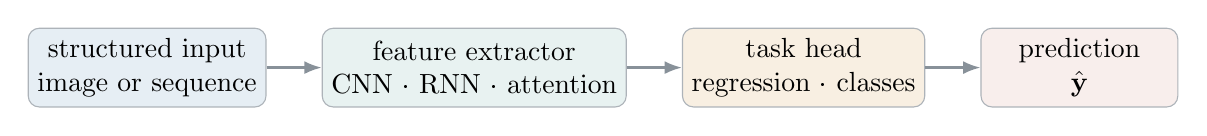
\begin{tikzpicture}[
    stage/.style={rounded corners, draw=softink!38, minimum width=2.5cm, minimum height=1.0cm, align=center},
    arrow/.style={-{Latex[length=2.2mm]}, thick, draw=softink!55}, node distance=0.7cm
  ]
    \node[stage, fill=softblue!15] (input) {structured input\\image or sequence};
    \node[stage, fill=softteal!15, right=of input] (features) {feature extractor\\CNN · RNN · attention};
    \node[stage, fill=softgold!18, right=of features] (head) {task head\\regression · classes};
    \node[stage, fill=softcoral!13, right=of head] (output) {prediction\\$\hat{\mathbf y}$};
    \draw[arrow] (input) -- (features);
    \draw[arrow] (features) -- (head);
    \draw[arrow] (head) -- (output);
  \end{tikzpicture}
  }
  \end{center}
  \begin{itemize}
    \item The output head and loss still follow Deck 01.
    \item What changes is how intermediate representations exchange information.
  \end{itemize}
\end{frame}

\sectiondivider{Convolutional Neural Networks}

\begin{frame}{Why Not Flatten an Image?\framecite{lecun1998}}
  An image $X\in\mathbb R^{C\times H\times W}$ has local and repeated structure.
  \begin{columns}[T]
    \column{0.48\textwidth}
    \begin{block}{Dense layer}
      \begin{itemize}
        \item forgets the grid after flattening
        \item separate weight for every pixel--unit pair
        \item $HWC\,d_{\text{out}}+d_{\text{out}}$ parameters
      \end{itemize}
    \end{block}
    \column{0.48\textwidth}
    \begin{block}{Convolutional layer}
      \begin{itemize}
        \item preserves spatial neighborhoods
        \item reuses each kernel across locations
        \item $k_hk_wC\,C_{\text{out}}+C_{\text{out}}$ parameters
      \end{itemize}
    \end{block}
  \end{columns}
  \vspace{0.25cm}
  Weight sharing makes a learned pattern detectable wherever it occurs.
\end{frame}

\begin{frame}{What Libraries Call Convolution}
  Deep-learning libraries normally implement cross-correlation:
  \[
    Y_{oij}=b_o+
    \sum_{c=1}^{C_{\mathrm{in}}}
    \sum_{u=0}^{k_h-1}\sum_{v=0}^{k_w-1}
    K_{ocuv}\,X_{c,\,is_h+u-p_h,\,js_w+v-p_w}.
  \]
  \begin{itemize}
    \item $o$: output channel; $c$: input channel
    \item $(i,j)$: output location; $(u,v)$: kernel location
    \item $s$: stride; $p$: zero padding
    \item Mathematical convolution additionally flips the kernel; learning works with either convention if it is used consistently.
  \end{itemize}
\end{frame}

\begin{frame}{A Worked Cross-Correlation}
  \begin{figure}
    \centering
    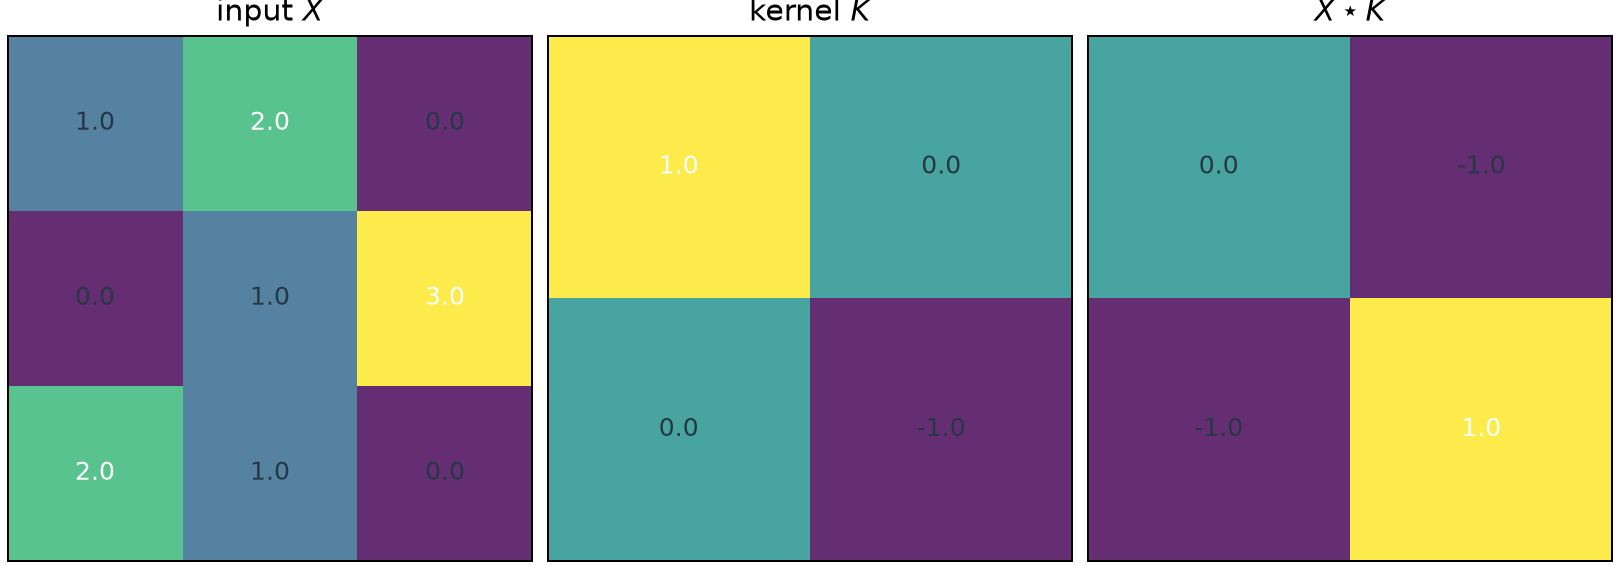
\includegraphics[width=0.78\linewidth]{convolution_walkthrough.png}
  \end{figure}
  \vspace{-0.3cm}
  The upper-left output is
  \[
    1(1)+2(0)+0(0)+1(-1)=0.
  \]
  The same four kernel parameters are reused for every output location.
\end{frame}

\begin{frame}{Channels Become Learned Feature Maps}
  \begin{center}
  \resizebox{0.96\linewidth}{!}{%
  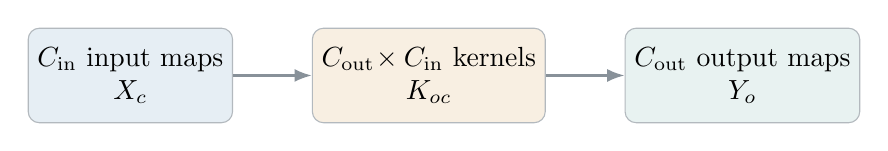
\begin{tikzpicture}[
    map/.style={draw=softink!35, rounded corners, minimum width=2.3cm, minimum height=1.2cm, align=center},
    arrow/.style={-{Latex[length=2.2mm]}, thick, draw=softink!55}, node distance=1.0cm
  ]
    \node[map, fill=softblue!15] (input) {$C_{\rm in}$ input maps\\$X_c$};
    \node[map, fill=softgold!18, right=of input] (kernels) {$C_{\rm out}\!\times C_{\rm in}$ kernels\\$K_{oc}$};
    \node[map, fill=softteal!15, right=of kernels] (output) {$C_{\rm out}$ output maps\\$Y_o$};
    \draw[arrow] (input) -- (kernels);
    \draw[arrow] (kernels) -- (output);
  \end{tikzpicture}
  }
  \end{center}
  \[
    Y_o=b_o+\sum_{c=1}^{C_{\rm in}} X_c\star K_{oc}.
  \]
  Early layers often respond to simple local patterns; later layers combine them into task-specific features.
\end{frame}

\begin{frame}{Output Size Is Determined, Not Guessed}
  For dilation one, one spatial dimension changes as
  \[
    H_{\rm out}=\left\lfloor
      \frac{H+2p-k}{s}
    \right\rfloor+1.
  \]
  \begin{exampleblock}{Example}
    $H=8$, $k=3$, $s=2$, $p=1$ gives
    \[
      H_{\rm out}=\left\lfloor\frac{8+2-3}{2}\right\rfloor+1=4.
    \]
  \end{exampleblock}
  \begin{itemize}
    \item ``same'' padding preserves size only for compatible choices of kernel and stride.
    \item Apply the same formula independently to width.
  \end{itemize}
\end{frame}

\begin{frame}{Parameter Sharing Changes the Scale}
  A $32\times32$ RGB image mapped to 64 outputs:
  \begin{columns}[T]
    \column{0.48\textwidth}
    \textcolor{softcoral}{\textbf{Dense mapping}}
    \[
      (32\cdot32\cdot3)\cdot64+64
      =196{,}672.
    \]
    \column{0.48\textwidth}
    \textcolor{softteal}{\textbf{$3\times3$ convolution}}
    \[
      3\cdot3\cdot3\cdot64+64
      =1{,}792.
    \]
  \end{columns}
  \vspace{0.35cm}
  \begin{block}{Trade-off}
    The CNN is much smaller because it assumes the same local pattern detector is useful across the grid.
  \end{block}
\end{frame}

\begin{frame}{Depth Grows the Receptive Field}
  \begin{columns}
    \column{0.58\textwidth}
    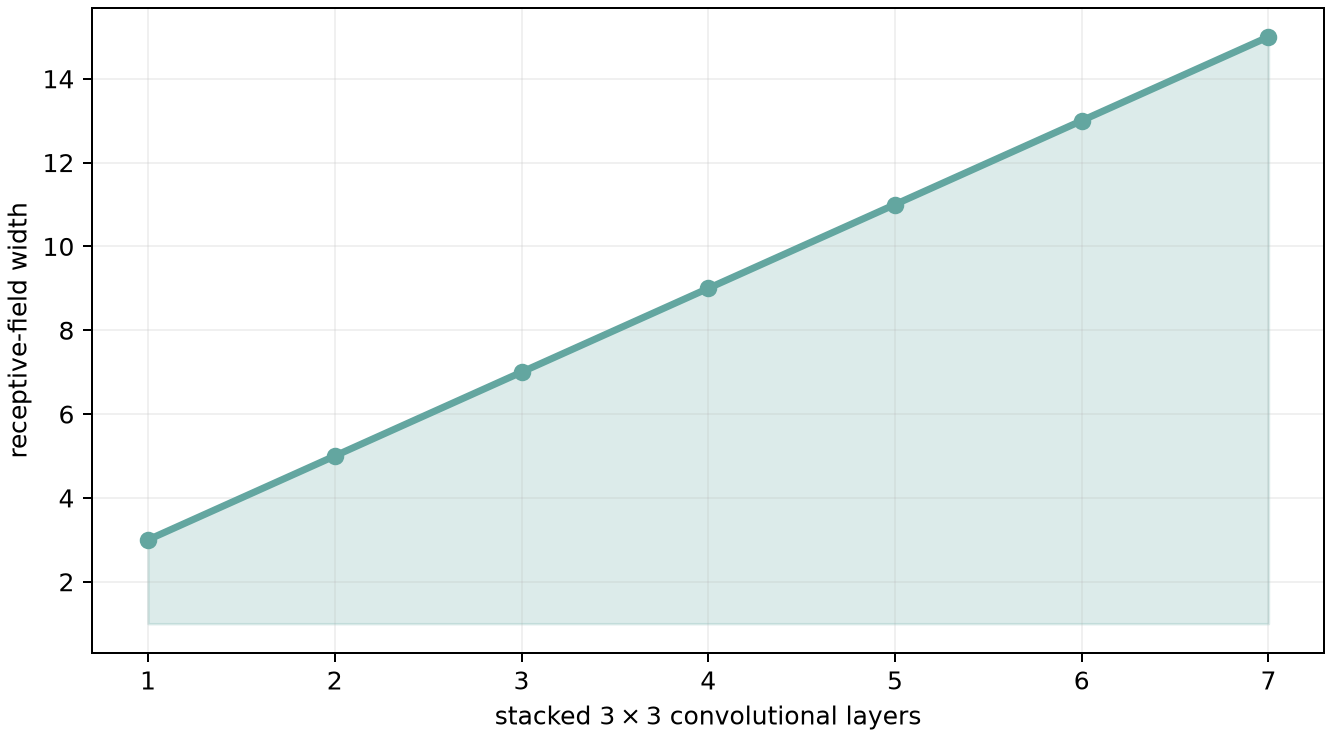
\includegraphics[width=\linewidth]{receptive_field_growth.png}
    \column{0.39\textwidth}
    For unit stride and no dilation, stacking $L$ kernels of width $3$ gives
    \[
      r_L=1+2L.
    \]
    Small kernels therefore build large-context features gradually while inserting nonlinearities between layers.
  \end{columns}
\end{frame}

\begin{frame}{A Practical CNN Pattern}
  \begin{center}
  \resizebox{0.96\linewidth}{!}{%
  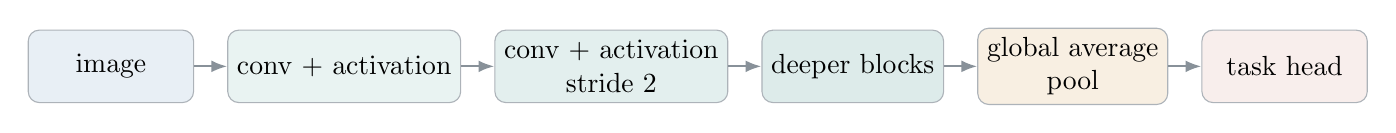
\begin{tikzpicture}[
    stage/.style={rounded corners, draw=softink!38, minimum width=2.1cm, minimum height=0.92cm, align=center},
    arrow/.style={-{Latex[length=2mm]}, thick, draw=softink!55}, node distance=0.42cm
  ]
    \node[stage, fill=softblue!14] (x) {image};
    \node[stage, fill=softteal!14, right=of x] (b1) {conv $+$ activation};
    \node[stage, fill=softteal!18, right=of b1] (b2) {conv $+$ activation\\stride $2$};
    \node[stage, fill=softteal!22, right=of b2] (b3) {deeper blocks};
    \node[stage, fill=softgold!18, right=of b3] (pool) {global average\\pool};
    \node[stage, fill=softcoral!13, right=of pool] (head) {task head};
    \foreach \a/\b in {x/b1,b1/b2,b2/b3,b3/pool,pool/head} \draw[arrow] (\a) -- (\b);
  \end{tikzpicture}
  }
  \end{center}
  \begin{itemize}
    \item Pooling or strided convolutions reduce spatial resolution.
    \item Global average pooling avoids a large fully connected layer tied to one image size.
    \item Residual connections are a later refinement, not required to understand convolution.
  \end{itemize}
\end{frame}

\sectiondivider{Recurrent Networks and Gated Memory}

\begin{frame}{A Recurrent Network Shares Parameters Across Time}
  \[
    \mathbf h_t=\tanh(W_x\mathbf x_t+W_h\mathbf h_{t-1}+\mathbf b_h),
    \qquad
    \hat{\mathbf y}_t=g(W_y\mathbf h_t+\mathbf b_y).
  \]
  \begin{itemize}
    \item $\mathbf h_t$ summarizes the prefix $\mathbf x_1,\ldots,\mathbf x_t$.
    \item The same $W_x,W_h,\mathbf b_h$ are reused at every time step.
    \item Outputs depend on the hidden state; they do not have to feed back as inputs.
    \item $g$ is chosen for the task: linear, sigmoid, or softmax.
  \end{itemize}
\end{frame}

\begin{frame}{Unrolling Reveals the Computation Graph}
  \begin{center}
  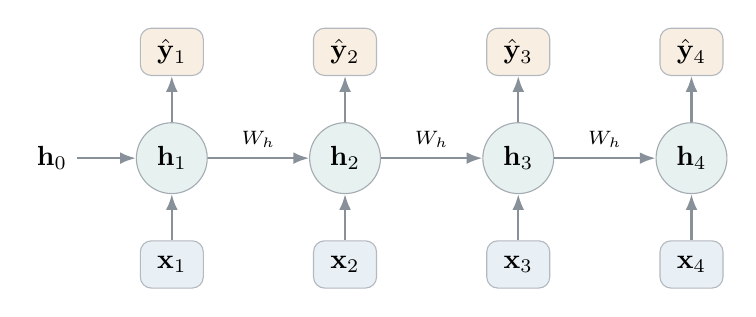
\begin{tikzpicture}[
    state/.style={circle, draw=softink!42, fill=softteal!16, minimum size=0.9cm},
    input/.style={rounded corners, draw=softink!35, fill=softblue!14, minimum width=0.8cm, minimum height=0.6cm},
    output/.style={rounded corners, draw=softink!35, fill=softgold!18, minimum width=0.8cm, minimum height=0.6cm},
    arrow/.style={-{Latex[length=2mm]}, thick, draw=softink!55}
  ]
    \foreach \t in {1,...,4} {
      \node[state] (h\t) at (2.2*\t,0) {$\mathbf h_{\t}$};
      \node[input] (x\t) at (2.2*\t,-1.35) {$\mathbf x_{\t}$};
      \node[output] (y\t) at (2.2*\t,1.35) {$\hat{\mathbf y}_{\t}$};
      \draw[arrow] (x\t) -- (h\t);
      \draw[arrow] (h\t) -- (y\t);
    }
    \foreach \a/\b in {1/2,2/3,3/4} \draw[arrow] (h\a) -- node[above, font=\scriptsize] {$W_h$} (h\b);
    \node[left=0.75cm of h1] (h0) {$\mathbf h_0$};
    \draw[arrow] (h0) -- (h1);
  \end{tikzpicture}
  \end{center}
  Backpropagation through time differentiates this unrolled graph. Parameter sharing lets sequences have variable length.
\end{frame}

\begin{frame}{Sequence Tasks Need Different Readouts}
  \centering
  \begin{tabular}{lll}
    \toprule
    Pattern & Example & Readout \\
    \midrule
    many-to-one & classify a vibration window & final or pooled hidden states \\
    many-to-many & forecast every future step & one output per time step \\
    encoder--decoder & map one sequence to another & decoded output sequence \\
    autoregressive & predict the next value/token & feed generated history forward \\
    \bottomrule
  \end{tabular}
  \par
  \vspace{0.45cm}
  Always state what is known at prediction time. A bidirectional encoder may process an entirely observed history window, but it must not encode inputs from the forecast horizon.
\end{frame}

\begin{frame}{Why Long Dependencies Are Difficult}
  With $J_j:=\partial\mathbf h_j/\partial\mathbf h_{j-1}$, repeated chain-rule factors appear across time:
  \[
    \frac{\partial\mathbf h_t}{\partial\mathbf h_k}
    =J_tJ_{t-1}\cdots J_{k+1}.
  \]
  \begin{columns}
    \column{0.58\textwidth}
    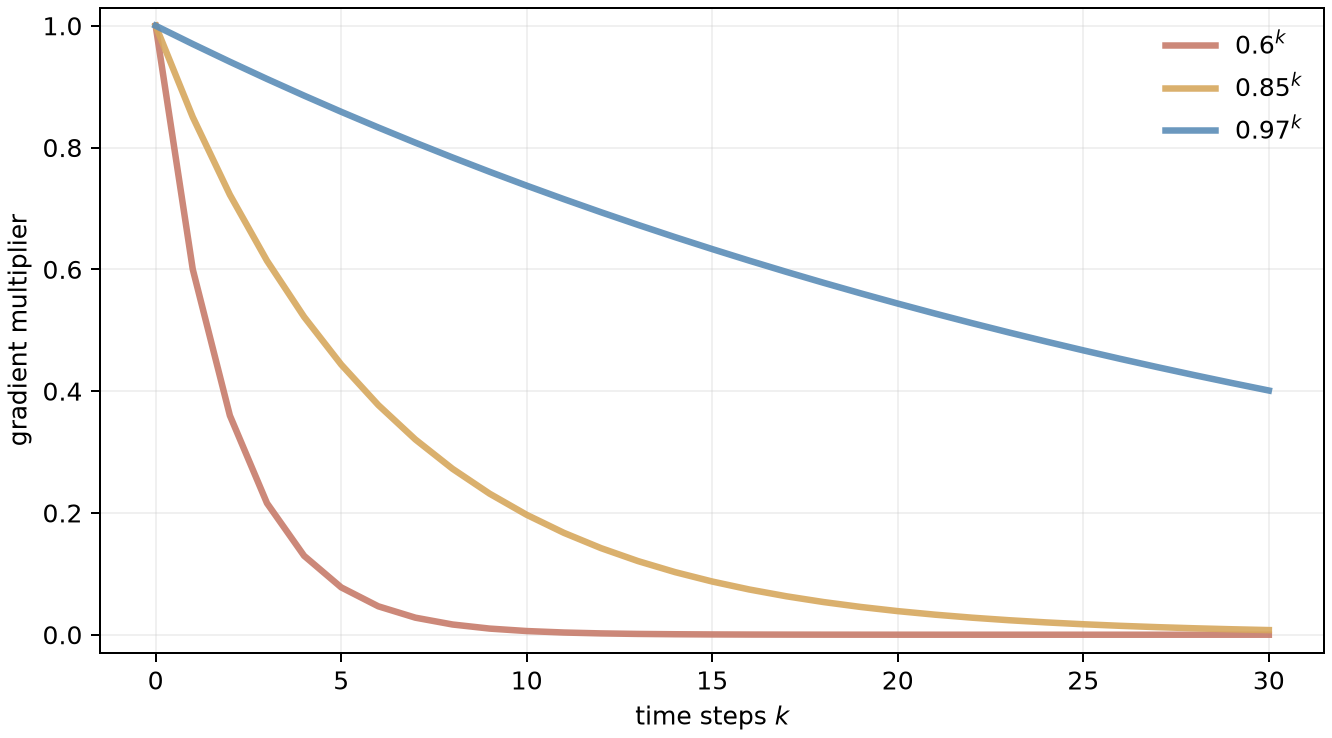
\includegraphics[width=\linewidth]{recurrent_gradient_decay.png}
    \column{0.39\textwidth}
    \begin{itemize}
      \item factors below one can make gradients vanish
      \item factors above one can make them explode
      \item gradient clipping limits explosions
      \item gated additive memory helps preserve information
    \end{itemize}
  \end{columns}
\end{frame}

\begin{frame}{LSTM: A Gated Additive Memory\framecite{hochreiter1997}}
  With $\mathbf u_t=[\mathbf x_t;\mathbf h_{t-1}]$:
  \[
    \mathbf f_t=\sigma(W_f\mathbf u_t+\mathbf b_f),\quad
    \mathbf i_t=\sigma(W_i\mathbf u_t+\mathbf b_i),
  \]
  \[
    \mathbf o_t=\sigma(W_o\mathbf u_t+\mathbf b_o),\quad
    \tilde{\mathbf c}_t=\tanh(W_c\mathbf u_t+\mathbf b_c),
  \]
  \[
    \mathbf c_t=\mathbf f_t\odot\mathbf c_{t-1}
      +\mathbf i_t\odot\tilde{\mathbf c}_t,
    \qquad
    \mathbf h_t=\mathbf o_t\odot\tanh(\mathbf c_t).
  \]
  All vectors have the hidden-state dimension; $\odot$ is element-wise multiplication.
\end{frame}

\begin{frame}{What the LSTM Gates Do}
  \begin{center}
  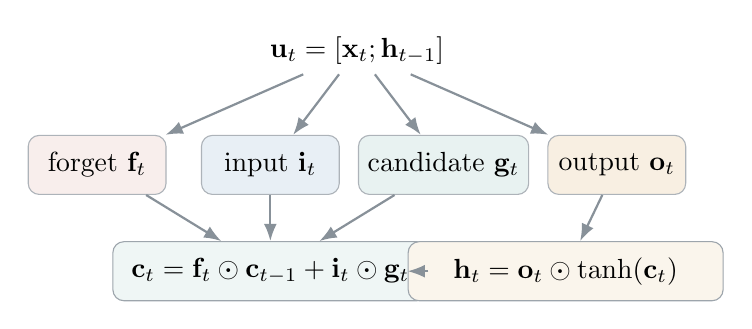
\begin{tikzpicture}[
    gate/.style={rounded corners, draw=softink!38, minimum width=1.75cm, minimum height=0.75cm, align=center},
    state/.style={rounded corners, draw=softink!45, minimum width=4.0cm, minimum height=0.75cm, align=center},
    arrow/.style={-{Latex[length=2.2mm]}, thick, draw=softink!55}
  ]
    \node (inputs) at (0,1.45) {$\mathbf u_t=[\mathbf x_t;\mathbf h_{t-1}]$};
    \node[gate, fill=softcoral!13] (forget) at (-3.3,0) {forget $\mathbf f_t$};
    \node[gate, fill=softblue!14] (input) at (-1.1,0) {input $\mathbf i_t$};
    \node[gate, fill=softteal!15] (candidate) at (1.1,0) {candidate $\mathbf g_t$};
    \node[gate, fill=softgold!18] (output) at (3.3,0) {output $\mathbf o_t$};
    \foreach \gate in {forget,input,candidate,output}{\draw[arrow] (inputs) -- (\gate);}
    \node[state, fill=softteal!10] (cell) at (-1.1,-1.35)
      {$\mathbf c_t=\mathbf f_t\odot\mathbf c_{t-1}+\mathbf i_t\odot\mathbf g_t$};
    \node[state, fill=softgold!12] (hidden) at (2.65,-1.35)
      {$\mathbf h_t=\mathbf o_t\odot\tanh(\mathbf c_t)$};
    \draw[arrow] (forget) -- (cell);
    \draw[arrow] (input) -- (cell);
    \draw[arrow] (candidate) -- (cell);
    \draw[arrow] (cell) -- (hidden);
    \draw[arrow] (output) -- (hidden);
  \end{tikzpicture}
  \end{center}
  \begin{itemize}
    \item Gates take values in $(0,1)$ and regulate information flow element by element.
    \item LSTMs improve long-range optimization but do not guarantee perfect memory.
  \end{itemize}
\end{frame}

\begin{frame}{When Recurrent Models Still Make Sense}
  \begin{itemize}
    \item streaming inference with a fixed-size state
    \item modest datasets where a compact model is useful
    \item low-latency sensor processing
    \item mechanical time-series forecasting, provided the split respects time and operating conditions
  \end{itemize}
  \begin{alertblock}{Evaluation warning}
    Randomly splitting overlapping windows can place nearly identical measurements in training and test sets. Split by trajectory, experiment, structure, or time first.
  \end{alertblock}
\end{frame}

\sectiondivider{Attention and Transformers}

\begin{frame}{Attention Is a Content-Dependent Weighted Average}
  For one query $\mathbf q$ and key--value pairs $(\mathbf k_j,\mathbf v_j)$:
  \[
    e_j=\frac{\mathbf q^\top\mathbf k_j}{\sqrt{d_k}},
    \qquad
    \alpha_j=\frac{\exp(e_j)}{\sum_r\exp(e_r)},
    \qquad
    \operatorname{Attn}(\mathbf q)=\sum_j\alpha_j\mathbf v_j.
  \]
  \begin{itemize}
    \item keys determine relevance to the query
    \item values carry the information being combined
    \item $\alpha_j\ge0$ and $\sum_j\alpha_j=1$
    \item the $\sqrt{d_k}$ scale prevents dot products from growing solely with dimension
  \end{itemize}
\end{frame}

\begin{frame}{Scaled Dot-Product Attention in Matrix Form\framecite{vaswani2017}}
  Given $X\in\mathbb R^{T\times d_{\rm model}}$:
  \[
    Q=XW_Q,\qquad K=XW_K,\qquad V=XW_V,
  \]
  \[
    \operatorname{Attention}(Q,K,V)
    =\operatorname{softmax}_{\rm row}
    \left(\frac{QK^\top}{\sqrt{d_k}}+M\right)V.
  \]
  \begin{itemize}
    \item $Q,K\in\mathbb R^{T\times d_k}$, $V\in\mathbb R^{T\times d_v}$
    \item $QK^\top\in\mathbb R^{T\times T}$ contains every query--key score
    \item mask $M$ is zero for allowed interactions and a large negative value for forbidden ones
  \end{itemize}
\end{frame}

\begin{frame}{Reading an Attention Matrix}
  \begin{columns}
    \column{0.59\textwidth}
    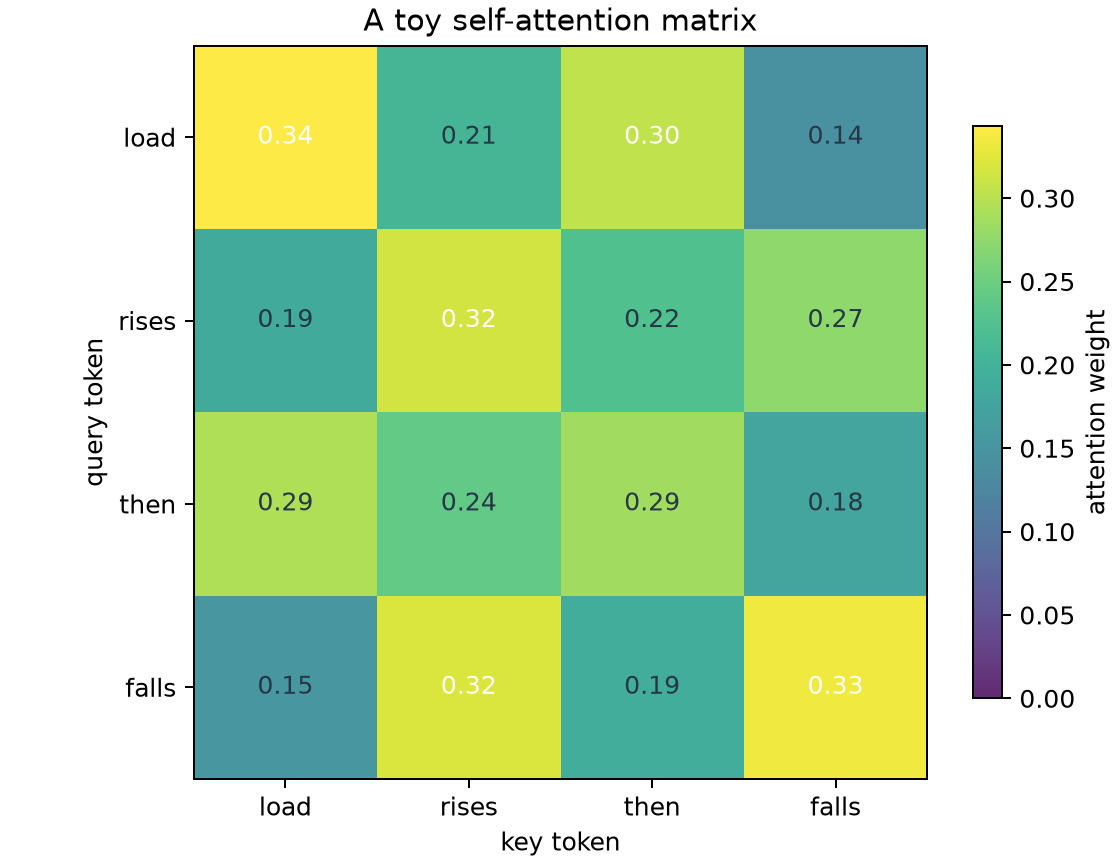
\includegraphics[width=\linewidth]{attention_heatmap.png}
    \column{0.38\textwidth}
    Each row answers:
    \begin{quote}
      For this query token, how much weight is assigned to every key token?
    \end{quote}
    Rows sum to one. Attention weights can aid inspection, but they are not automatically causal explanations.
  \end{columns}
\end{frame}

\begin{frame}{Self-Attention Needs Position Information}
  Without positional information, self-attention treats a permutation of the input as the same set of tokens.
  \[
    X_0=E_{\rm token}+E_{\rm position}.
  \]
  \begin{itemize}
    \item sinusoidal encodings provide deterministic positions
    \item learned position embeddings are optimized with the model
    \item relative-position methods encode distances between tokens
  \end{itemize}
  \begin{block}{Key distinction}
    Attention decides \emph{which content interacts}; position encodings tell the model \emph{where that content occurs}.
  \end{block}
\end{frame}

\begin{frame}{Multi-Head Attention Learns Several Relations}
  \[
    \operatorname{head}_r
    =\operatorname{Attention}(XW_Q^{(r)},XW_K^{(r)},XW_V^{(r)}),
  \]
  \[
    \operatorname{MHA}(X)
    =\operatorname{Concat}(\operatorname{head}_1,\ldots,\operatorname{head}_h)W_O.
  \]
  \begin{itemize}
    \item Every head has its own learned projections.
    \item Heads can represent different interaction patterns.
    \item More heads do not guarantee more interpretable or independent relations.
  \end{itemize}
\end{frame}

\begin{frame}{A Transformer Block\framecite{vaswani2017}}
  \begin{center}
  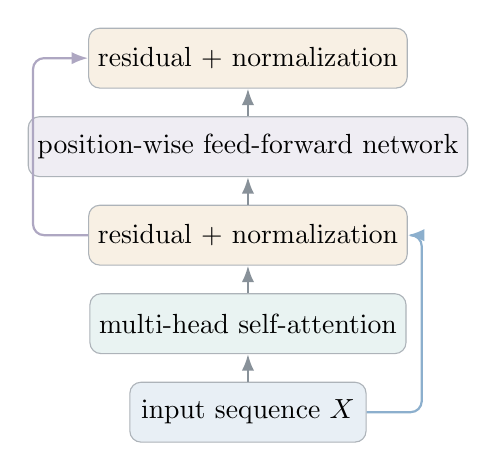
\begin{tikzpicture}[
    stage/.style={rounded corners, draw=softink!38, minimum width=3.0cm, minimum height=0.76cm, align=center},
    arrow/.style={-{Latex[length=2.1mm]}, thick, draw=softink!55}, node distance=0.35cm
  ]
    \node[stage, fill=softblue!14] (x) {input sequence $X$};
    \node[stage, fill=softteal!14, above=of x] (attn) {multi-head self-attention};
    \node[stage, fill=softgold!17, above=of attn] (add1) {residual $+$ normalization};
    \node[stage, fill=softpurple!14, above=of add1] (ffn) {position-wise feed-forward network};
    \node[stage, fill=softgold!17, above=of ffn] (add2) {residual $+$ normalization};
    \draw[arrow] (x) -- (attn);
    \draw[arrow] (attn) -- (add1);
    \draw[arrow] (add1) -- (ffn);
    \draw[arrow] (ffn) -- (add2);
    \draw[arrow, rounded corners, draw=softblue!70] (x.east) -- ++(0.7,0) |- (add1.east);
    \draw[arrow, rounded corners, draw=softpurple!70] (add1.west) -- ++(-0.7,0) |- (add2.west);
  \end{tikzpicture}
  \end{center}
  Residual paths preserve information and provide short gradient routes; normalization stabilizes activation scales.
\end{frame}

\begin{frame}{Causal Masking Prevents Looking Ahead}
  For autoregressive prediction at position $t$, allow keys only from positions $j\le t$:
  \[
    M_{tj}=\begin{cases}
      0, & j\le t,\\
      -\infty, & j>t.
    \end{cases}
  \]
  After the row-wise softmax, masked positions receive zero weight.
  \begin{alertblock}{Leakage warning}
    A forecasting transformer without a causal mask can use future targets during training and appear unrealistically accurate.
  \end{alertblock}
\end{frame}

\begin{frame}{Three Common Transformer Families}
  \centering
  \small
  \begin{tabular}{llll}
    \toprule
    Family & Visible context & Typical use & Example pattern \\
    \midrule
    encoder-only & both directions & representation, classification & BERT-like \\
    decoder-only & past positions & autoregressive generation & GPT-like \\
    encoder--decoder & input + decoded past & sequence-to-sequence & translation \\
    \bottomrule
  \end{tabular}
  \par
  \vspace{0.45cm}
  These are masking and connectivity choices, not three unrelated mathematical models.
\end{frame}

\begin{frame}{RNN or Transformer?}
  \centering
  \begin{tabular}{lll}
    \toprule
    Property & RNN/LSTM & Full self-attention \\
    \midrule
    time-step computation & sequential & parallel during training \\
    persistent state & fixed-size hidden state & stores all token representations \\
    long-range path & grows with distance & one attention edge \\
    sequence cost & $O(T)$ recurrent steps & $O(T^2)$ score matrix \\
    streaming & natural & needs caching or restricted attention \\
    \bottomrule
  \end{tabular}
  \par
  \vspace{0.4cm}
  The best choice depends on sequence length, latency, data volume, and hardware—not fashion.
\end{frame}

\begin{frame}{Architecture Map and Course Boundaries}
  \begin{itemize}
    \item \textcolor{softblue}{\textbf{MLP:}} fixed-size vectors; dense feature mixing
    \item \textcolor{softteal}{\textbf{CNN:}} grids; local shared kernels
    \item \textcolor{softgold}{\textbf{RNN/LSTM:}} sequences; recurrent state and gated memory
    \item \textcolor{softpurple}{\textbf{Transformer:}} sequences or sets; content-dependent interactions
    \item \textcolor{softcoral}{\textbf{GNN:}} irregular relational data; continue in Deck 04
  \end{itemize}
  \begin{block}{Next}
    All these architectures are compositions of differentiable operations. Deck 03 explains losses, backpropagation, optimization, and generalization. Generative objectives belong to Deck 07.
  \end{block}
\end{frame}

\end{document}
